% Formula sheet for MEC E 371 Heat Transfer
% Two column format

\documentclass[10pt]{article}
\usepackage{amsmath}
\usepackage{amssymb}
\usepackage{multicol}
\usepackage{geometry}
\usepackage{fancyhdr}
\usepackage{siunitx}
\usepackage{enumitem}
\usepackage{multicol}
\usepackage{graphicx}
\usepackage{multirow}
\usepackage{lastpage}
\usepackage[final]{hyperref}
\usepackage{parskip}

\geometry{letterpaper, portrait, margin=0.5in, footskip=0.25in, top = 0.75in, headsep=0.25in}
\setlength{\columnsep}{0.5in}

\hypersetup{
	colorlinks=true,       % false: boxed links; true: colored links
	linkcolor=blue,        % color of internal links
	citecolor=blue,        % color of links to bibliography
	filecolor=magenta,     % color of file links
	urlcolor=blue         
}

\pagestyle{fancy}
\fancyhf{}
\lhead{MEC E 371 Formula Sheet}
\chead{Last Updated: \today}
\rhead{Alex Diep}
\cfoot{\thepage\ of \pageref{LastPage}}

\begin{document}
%\maketitle
%\thispagestyle{empty}
\begin{multicols*}{2}
\section*{8. Internal Forced Convection}
\subsection*{8.1. General Procedure}
\begin{enumerate}
    \item Find fluid properties from Appendix 1 at bulk mean temperature $T_b = (T_i + T_e)/2$
    \begin{itemize}
        \item $\rho$, $\mu$, $k$, $c_p$, $Pr$, $\nu$
    \end{itemize}
    \item Determine mean velocity $V_{\text{avg}}$
    \item Determine the type of flow (laminar or turbulent)
    \begin{itemize}
        \item Laminar: Re $< 2300$
        \item Turbulent: Re $> 4000$
    \end{itemize}
    \item Determine the Nusselt number, Nu, using the appropriate correlation
    \begin{itemize}
        \item Check if $l_{h, \text{laminar}}$ and $l_{t, \text{laminar}}$ is less than $L$. If so, use Table \ref{tab:sec8_fully_developed_laminar} 
        \item Else, use empirical correlations
    \end{itemize}
    \item Determine the heat transfer coefficient $h$ using $Nu$, $k$, and $A_s$
\end{enumerate}

% Add this to a glossary section later
\subsection*{8.2. Variable Definitions}
\begin{itemize}
    \item Nu: Nusselt number
    \item Re: Reynolds number
    \item Pr: Prandtl number
    \item $\mu$: Dynamic viscosity
    \item $\nu$: Kinematic viscosity
    \item $k$: Thermal conductivity
    \item $h$: Convection heat transfer coefficient
    \item $D_h$: Hydraulic diameter
    \item $A_s$: Surface area
    \item $A_c$: Cross-sectional area
    \item $V_{\text{avg}}$: Average velocity
    \item $T_b$: Bulk mean temperature
    \item $T_i$: Inlet temperature
    \item $T_e$: Exit temperature
    \item $\dot{m}$: Mass flow rate
    \item $\dot{q}$: Heat flux 
    \item $\Delta T_{\text{lm}}$: Log mean temperature difference   
\end{itemize}

\subsection*{8.3. Formulas}
\vspace{-0.4cm}
\begin{align*}
    \dot{m} &= \rho V_{\text{avg}} A_c \\
    \text{Re} &= \frac{\rho V_{\text{avg}} D_h}{\mu}  = \frac{V_{\text{avg}} D_h}{\nu} \\
    D_h &= \frac{4 A_c}{\text{Perimeter}} = D\rvert_{\text{circular}} = a\rvert_{\text{square}}   \\
    &= \frac{2ab}{a + b} \bigg\rvert_{\text{rectangular}} = \frac{4ab}{a+b}\bigg\rvert_{\text{channel}} \\
    \text{Nu} &= \frac{hD_h}{k} \\ 
    A_s &= \pi D L|_{\text{circular}} = 4ab|_{\text{rectangular}} \\
    A_c &= \pi \frac{D^2}{4}|_{\text{circular}} = ab|_{\text{rectangular}} \\
    l_{h, \text{laminar}} &= 0.05 \text{Re} D_h \\
    l_{t, \text{laminar}} &= 0.05 \text{Re} \text{Pr} D_h = \text{Pr} l_{h, \text{laminar}} \\
    l_{h, \text{turbulent}} &\approx l_{t, \text{turbulent}} = 10D_h 
\end{align*}
\vspace{-0.5cm}
Constant $\dot{q}$:
\begin{align*}
    T_e &= T_i + \frac{\dot{q}}{\dot{m} c_p} \\ 
    \dot{q} = h(T_s-T_b)
\end{align*}
Constant $T_s$:
\vspace{-0.5cm}
\begin{align*}
    T_e &= T_s - (T_s - T_i) \exp\left(-\frac{h A_s}{\dot{m} c_p}\right) \\
    T_s &=\frac{T_e - T_i \exp\left(-\frac{\dot{m} C_p}{h A_s}\right)}{1 - \exp\left(-\frac{\dot{m} C_p}{h A_s}\right)} \\
    \dot{Q} &= h A_s \Delta T_{\text{lm}} \\
    T_{\text{lm}} &= \frac{T_{i} - T_{e}}{\ln[(T_{s} - T_{e})/(T_{s} - T_{i})]} 
\end{align*}    
For fully developed laminar flow, use Table \ref{tab:sec8_fully_developed_laminar}.

For entry region in a circular tube where $T_s = \text{constant}$, use:
\vspace{-0.5cm}
\begin{align*}
    \text{(Edwards et al., 1979) } \text{Nu} = 3.66 + \frac{0.0658(D/L) \text{Re} \text{Pr}}{1 + 0.04[(D/L) \text{Re} \text{Pr}]^{2/3}} 
\end{align*}

For entry region in a circular tube where the difference between $T_s$ and $T_b$ is large, use:
\vspace{-0.3cm}
\begin{align*}
    \text{(Sieder and Tate, 1936) } &\text{Nu} = 1.86\left(\frac{\text{Re} \text{Pr} D}{L}\right)^{1/3} \left(\frac{\mu_b}{\mu_s}\right)^{0.14} \\
    0.6 < \text{Pr} < 5, &\quad 0.0044 < \frac{\mu_b}{\mu_s} < 9.75
\end{align*}
All properties for Sieder and Tate should be evaluated at $T_b$ except $\mu_s$ which should be evaluated at $T_s$.

For entry region between two isothermal parallel plates, use:
\vspace{-0.3cm}
\begin{align*}
    \text{(Edwards et al., 1979) } &\text{Nu} = 7.54 + \frac{0.03(D_h/L) \text{Re} \text{Pr}}{1 + 0.016[(D_h/L) \text{Re} \text{Pr}]^{2/3}} \\
    &\text{Re} \leq 2800
\end{align*}
For turbulent flow in a circular tube, use:
\vspace{-0.3cm}
\begin{align*}
    \text{(Dittus-Boelter, 1930) } \text{Nu} = 0.023 \text{Re}^{0.8} \text{Pr}^{n}  \\
    n = 0.4 \; (\text{Heating}), \quad n = 0.3 \; (\text{Cooling}) 
\end{align*}
% Pressure drop:\footnote{Check if $D_h$ should be used for $D$ in $V_{\text{avg}}$. Also I don't think he covers this in class.}
% \begin{align*}
%     \Delta P_{L} &= f \frac{L}{D_h} \frac{\rho V_{\text{avg}}^2}{2} \\
%     h_L &= \frac {\Delta P_L}{\rho g} = f \frac{L}{D_h} \frac{V_{\text{avg}}^2}{2g} \\
%     f|_{\text{laminar}} &= \frac{64}{\text{Re}} \\
%     V_{\text{avg}} &= \frac{\Delta P D^2}{32 \mu L} \\
% \end{align*} 
\end{multicols*}

\section*{Tables}
\begin{table}[h]
    \centering
    \caption{Nusselt number and friction factor for fully developed laminar flow in tubes of various cross sections 
    ($D_h = 4A_c /P$, $Re = V_{\text{avg}} D_h / \nu$, and $\text{Nu} = hD_h / k$) (\textbf{Table 8-1 in textbook})}
    \label{tab:sec8_fully_developed_laminar}
    \begin{tabular}{ccccc}
        \hline
        & & \multicolumn{2}{c}{Nu} & \\
        \cline{3-4}
        Tube Geometry & $a/b$ or $\theta^\circ$ & $T_s = \text{constant}$ & $\dot{q}_s = \text{constant}$ & $f$ \\
        \hline
        \raisebox{-\totalheight}{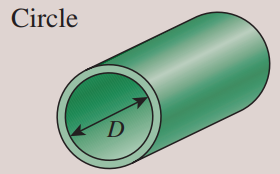
\includegraphics[width=0.15\textwidth]{Figures/Sec8 Circle Fully Laminar.png}} & --- & 4.36 & 3.66 & 64/Re \\
        \hline
        & \underline{$a/b$} & & & \\ 
        \multirow{2}{*}{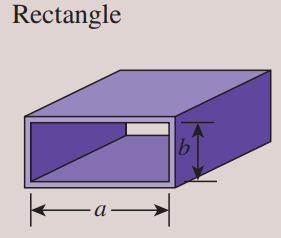
\includegraphics[width=0.15\textwidth]{Figures/Sec8 Rectangle Fully Laminar.png}} 
        & 1 & 2.98 & 3.61 & 56.92/Re \\
        & 2 & 3.39 & 4.12 & 62.20/Re \\
        & 3 & 3.96 & 4.79 & 68.36/Re \\
        & 4 & 4.44 & 5.33 & 72.92/Re \\
        & 6 & 5.14 & 6.05 & 78.80/Re \\
        & 8 & 5.60 & 6.49 & 82.32/Re \\
        & $\infty$ & 7.54 & 8.24 & 96.00/Re \\
        \hline
        & \underline{$a/b$} & & & \\
        \multirow{2}{*}{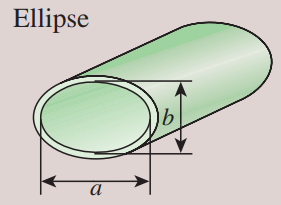
\includegraphics[width=0.15\textwidth]{Figures/Sec8 Ellipse Fully Laminar.png}}
        & 1 & 3.66 & 4.36 & 64.00/Re \\
        & 2 & 3.74 & 4.56 & 67.28/Re \\
        & 4 & 3.79 & 4.88 & 72.96/Re \\
        & 8 & 3.72 & 5.09 & 76.60/Re \\
        & 16 & 3.65 & 5.18 & 78.16/Re \\
        \hline
        & \underline{$\theta^\circ$} & & & \\
        \multirow{2}{*}{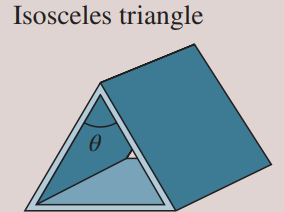
\includegraphics[width=0.15\textwidth]{Figures/Sec8 Triangle Fully Laminar.png}}
        & 10 & 1.61 & 2.45 & 50.80/Re \\
        & 30 & 2.26 & 2.91 & 52.28/Re \\
        & 60 & 2.47 & 3.11 & 53.32/Re \\
        & 90 & 2.34 & 2.98 & 52.60/Re \\
        & 120 & 2.00 & 2.68 & 50.96/Re \\
        \hline
        % \raisebox{-\totalheight}{\includegraphics[width=0.15\textwidth]{Figures/Sec8 Square Fully Laminar.png}} & 1 & 3.66 & 3.11 & 64/Re \\
    \end{tabular}
\end{table}

% a/b
% 1
% 2
% 3
% 4
% 6
% 8
% ∞
% 2.98
% 3.39
% 3.96
% 4.44
% 5.14
% 5.60
% 7.54
% 3.61
% 4.12
% 4.79
% 5.33
% 6.05
% 6.49
% 8.24
% 56.92/Re
% 62.20/Re
% 68.36/Re
% 72.92/Re
% 78.80/Re
% 82.32/Re
% 96.00/Re
% Ellipse a/b
% 1
% 2
% 4
% 8
% 16
% 3.66
% 3.74
% 3.79
% 3.72
% 3.65
% 4.36
% 4.56
% 4.88
% 5.09
% 5.18
% 64.00/Re
% 67.28/Re
% 72.96/Re
% 76.60/Re
% 78.16/Re
% Isosceles triangle θ
% 10°
% 30°
% 60°
% 90°
% 120°
% 1.61
% 2.26
% 2.47
% 2.34
% 2.00
% 2.45
% 2.91
% 3.11
% 2.98
% 2.68
% 50.80/Re
% 52.28/Re
% 53.32/Re
% 52.60/Re
% 50.96/Re

\end{document}
